\documentclass[reprint,
%superscriptaddress,
%groupedaddress,
%unsortedaddress,
%runinaddress,
%frontmatterverbose, 
%preprint,
%preprintnumbers,
nofootinbib,
%nobibnotes,
%bibnotes,
amsmath,amssymb,
aps]{revtex4-1}
\usepackage{physics}
\usepackage{graphicx}
\usepackage{amsmath}
\usepackage{subfigure}
\usepackage{bm}
\usepackage{dcolumn}% Align table columns on decimal point
\usepackage{framed}
\usepackage{empheq}
\usepackage{amsfonts}
\usepackage{esint}
\usepackage[makeroom]{cancel}
\usepackage{dsfont}
\usepackage{centernot}
\usepackage{mathtools}
\usepackage{bigints}
\usepackage{empheq}
\usepackage{tensor}
\usepackage{xcolor}
\definecolor{colby}{rgb}{0.0, 0.0, 0.5}
\definecolor{MIT}{RGB}{163, 31, 52}
\usepackage[pdftex]{hyperref}
%\hypersetup{colorlinks,linkcolor={MIT},citecolor={MIT},urlcolor={MIT}}  
\hypersetup{colorlinks,linkcolor=blue,citecolor=blue,urlcolor=blue}  
%\usepackage[left=1in,right=1in,top=1in,bottom=1in]{geometry}
%\setcounter{MaxMatrixCols}{20}
% \usepackage{newpxtext,newpxmath}
%\newcommand*\widefbox[1]{\fbox{\hspace{2em}#1\hspace{2em}}}

\newcommand{\p}{\partial}
\newcommand{\R}{\mathbb{R}}
\newcommand{\C}{\mathbb{C}}
\newcommand{\lag}{\mathcal{L}}
\newcommand{\nn}{\nonumber}
\newcommand{\ham}{\mathcal{H}}
\newcommand{\M}{\mathcal{M}}
\newcommand{\I}{\mathcal{I}}
\newcommand{\K}{\mathcal{K}}
\newcommand{\F}{\mathcal{F}}
\newcommand{\w}{\omega}
\newcommand{\lam}{\lambda}
\newcommand{\al}{\alpha}
\newcommand{\be}{\beta}
\newcommand{\x}{\xi}
\newcommand{\G}{\mathcal{G}}
\newcommand{\f}[2]{\frac{#1}{#2}}
\newcommand{\ift}{\infty}
\newcommand{\lp}{\left(}
\newcommand{\rp}{\right)}
\newcommand{\lb}{\left[}
\newcommand{\rb}{\right]}
\newcommand{\lc}{\left\{}
\newcommand{\rc}{\right\}}
\newcommand{\V}{\mathbf{V}}
\newcommand{\U}{\mathcal{U}}
\newcommand{\Id}{\mathcal{I}}
\newcommand{\D}{\mathcal{D}}
\newcommand{\Z}{\mathcal{Z}}

\definecolor{gris245}{RGB}{245,245,245}
\definecolor{olive}{RGB}{50,140,50}
\definecolor{brun}{RGB}{175,100,80}

\newcommand{\diag}{\text{diag}}
\newcommand{\psirot}{\ket{\psi_\text{rot}(t)} }
\newcommand{\RWA}{\ham_\text{rot}^\text{RWA}}

% 3j symbol
\newcommand{\tj}[6]{ \begin{pmatrix}
		#1 & #2 & #3 \\
		#4 & #5 & #6 
\end{pmatrix}}



\begin{document}
	
	

\title{Berry Phase and Atom Interferometry\\with Applications to an Observation of the Gravitational Aharonov-Bohm Effect}
\author{Huan Q. Bui}
\email{huanbui@mit.edu}
\affiliation{
	MIT-Harvard Center for Ultracold Atoms, Research Laboratory of Electronics, and Department of Physics, Massachusetts Institute of Technology, Cambridge, Massachusetts 02139, USA}
\date{\today}


\begin{abstract}
	Following the conception of the Aharonov-Bohm effect due to Ehrenberg, Siday, Aharonov, and Bohm in the mid-20$^\text{th}$ century, experimental verifications of the effect emerged in the late 1980s and opened up developments in matter-wave interferometry. Starting in the 1990s, interests in atom interferometry grew as physicists realized the atom's remarkable ability as a quantum sensor. In this paper, we review the notion of Berry phase and interpret the Aharonov-Bohm effect as an example. Then, we review the principles of atom interferometry, specifically two atom-light interactions which are instrumental to modern atom interferometers. Finally, we briefly survey and contextualize a recent observation of the gravitational analogue of the Aharonov-Bohm effect. 
%	\begin{description}
%		\item[Keywords]
%		Berry phase, Aharonov-Bohm effect, Atom interferometry 
%	\end{description}
\end{abstract}

%\keywords{Suggested keywords}%Use showkeys class option if keyword
%display desired

\maketitle

%\tableofcontents



\section{Introduction}




The outline of this paper is as follows.  Section \ref{sect:berry} is a review of the Berry phase and the Aharonov-Bohm effect. While these are standard topics in many quantum mechanics texts (see, for example, \cite{shankar2012principles}, \cite{griffiths2018introduction}, \cite{sakurai1995modern}), there is a wide variability in the style and context in which they are presented. It is therefore beneficial to provide a self-contained exposition here, to have the theory right at our fingertips. Section \ref{sect:atom} reviews the principles of atom interferometry, with an emphasis on two atom-light interactions that are crucial for modern atom interferometers: stimulated Raman transitions and Bragg diffraction. Section \ref{sect:grav} briefly reviews the recent observation of the gravitational analogue of the Aharonov-Bohm effect due to Overstreet \textit{et al.} \cite{overstreet2022observation}.



\section{Berry phase}\label{sect:berry}
Consider $\mathcal{H}(\bm{R}(t))$, a Hamiltonian parameterized by a family of variables $\bm{R}(t)$. Let $\ket{\psi(0)} = \ket{n(\bm{R}(0))}$, the $n^\text{th}$ eigenstate of $\mathcal{H}(\bm{R}(0))$. By the adiabatic theorem, $\ket{\psi(t)}$ is $\ket{n(\bm{R}(t))}$, the $n^\text{th}$ instantaneous eigenstate of $\mathcal{H}(t)$, up to a phase factor:
\begin{align*}
\ket{\psi(t)} = e^{ -\f{i}{\hbar }\int_0^t E_n(\bm{R} (t'))\,dt' } \exp(i\gamma_n(t)) \ket{n(\bm{R}(t))},
\end{align*}
where $\gamma_n(t)$ is called the \textit{Berry phase}. From the Schr\"{o}dinger equation for $\ket{\psi(t)}$, we have
\begin{align*}
\dot{\gamma}_n(t) = i \bra{n(\bm{R}(t))} \nabla_{\bm{R}}  \ket{n(\bm{R}(t)) } \cdot \dot{\bm{R}}(t).
\end{align*}
In particular, at some final time $t_f$,
\begin{align}\label{eq:def}
\gamma_n(t_f) =   \int^{\bm{R}_f}_{\bm{R}_i} i \bra{n(\bm{R})} \nabla_{\bm{R}}  \ket{n(\bm{R}) } \cdot d{\bm{R}},
\end{align} 
which depends only on the path taken in parameter space. Define the \textit{Berry connection}, 
\begin{align*}
\bm{A}_n(\bm{R}) = i \bra{n(\bm{R})} \nabla_{\bm{R}}  \ket{n(\bm{R}) }
\end{align*} 
and consider gauge transformation in parameter space of instantaneous eigenstates $\ket{n(\bm{R})} \to \ket{\widetilde{n}(\bm{R})} = e^{-i\beta(\bm{R})}\ket{n(\bm{R})}$. The Berry connection transforms like the electromagnetic  vector potential:
\begin{align*}
\bm{A}_n(\bm{R}) \to  \widetilde{\bm{A}_n}(\bm{R}) = \bm{A}_n(\bm{R}) + \nabla_{\bm{R}} \beta (\bm{R}),
\end{align*}
while the Berry phase transforms as
\begin{align*}
\widetilde{\gamma_n} (\bm{R}) = \int_{\bm{R}_i}^{\bm{R}_f} \widetilde{A_n}(\bm{R})\cdot d\bm{R} = \gamma_n(\bm{R}_f)  + \beta(\bm{R}_f) - \beta({\bm{R}_i}),
\end{align*}
which is gauge-invariant exactly when the Hamiltonian evolution is cyclical, i.e., $\bm{R}(t_f) = \bm{R}(0)$. In such a case, the Berry phase is well-defined and measurable by means of interferometry.\footnote{There is also the notion of the \textit{Berry curvature}, but it is not relevant to the scope of this paper.}

%The Berry phase depends on the topology of the parameter space containing the path $C$. Let $\mathfrak{R}$ denote the parameter space. If $\mathfrak{R}$ is one-dimensional, the Berry phase vanishes. If $\mathfrak{R}$ is three-dimensional, 
%\begin{align*}
%\gamma_n(C) &=  \oint_C \bm{A}_n(\bm{R}) \cdot d{\bm{R}} \\
%&= \iint_{S} \lb  \nabla_{\bm{R}} \times \bm{A}_n(\bm{R}) \rb  \cdot d\vec{S} \equiv \iint_S \bm{D}_n \cdot d\vec{S}
%\end{align*}
%by Stokes' theorem, where $S$ is the surface with boundary $C$ and $\bm{D}_n \equiv \nabla_{\bm{R}} \times \bm{A}(\bm{R}) $ is the \textit{Berry curvature}. 

%We immediately see that if we think of the Berry connection as the electromagnetic vector potential, then the Berry curvature plays the role of the associated magnetic field, which is gauge-invariant.



%\subsection{Example: Spin-1/2 in a magnetic field}
%
%The Hamiltonian for a spin-1/2 in a magnetic field is
%\begin{align*}
%\mathcal{H}(\bm{B}) = \bm{B}\cdot \bm{\sigma} = r \begin{pmatrix}
%\cos\theta & \sin\theta e^{-i\phi} \\ \sin\theta e^{i\phi} & -\cos\theta
%\end{pmatrix}.
%\end{align*}
%The eigenvalues are $\pm r$, with associated eigenvectors
%\begin{align*}
%\ket{+} = \begin{pmatrix}
%\cos(\theta/2) \\ e^{i\phi}\sin(\theta/2) 
%\end{pmatrix}, \quad \ket{-} = \begin{pmatrix}
%\cos(\theta/2) \\ - e^{i\phi}\sin(\theta/2) 
%\end{pmatrix} .
%\end{align*}
%We require that $r  \neq 0$ for the adiabatic theorem to hold. The components of the Berry connection for $\ket{+}$ are readily calculated:
%\begin{align*}
%&A_r = i\bra{+}\p_r \ket{+} = 0\\
%&A_\theta = i\bra{+}\p_\theta\ket{+} = 0\\
%&A_\phi = i\bra{+}\p_\phi \ket{+} = (\cos\theta - 1)/2.
%\end{align*}
%Consider a closed, piece-wise smooth path $C$ enclosing a surface $S$ such that no point of $S$ lies on the negative $z$-axis\footnote{Here, $\bm{A}(\bm{B})$ is actually not defined on the negative $z$-axis.}. The Berry phase is 
%\begin{align*}
%\gamma[C] = \oint_C \bm{A}(\bm{B}) \cdot d\bm{B} = \iint_S \nabla \times \bm{A}(\bm{B})  \, d\bm{S} = -\f{\Omega}{2} 
%\end{align*}
%where $\Omega$ is nothing but the solid angle enclosed by $S$. If we had chosen the $z$-axis to lie in the opposite direction, then the solid angle would have been $|\Omega'| = 4\pi - |\Omega|$.  While this appears problematic,  $\exp(i\gamma[C])$ is the same in both cases, and the Berry phase is still well-defined. 




\subsection{Aharonov-Bohm Effect}


The Aharonov-Bohm effect is often discussed in the context of the path integral formulation of quantum mechanics.  Here, the author presents M. V. Berry's interpretation of the Aharonov-Bohm effect as a Berry phase change in a more traditional quantum mechanical language.
%\footnote{The presentation due to \cite{griffiths2018introduction}, based on Berry's paper \cite{berry1984quantal}, fills in mathematical steps skipped by Berry and is highly pedagogical.}. 
This is not only an illustrative application of \eqref{eq:def}, but also avoids issues with single-valuedness of wavefunctions that arise in \cite{aharonov1959significance} and \cite{ehrenberg1949refractive} as suggested by Berry. 



%\begin{figure}
%	\includegraphics[width=0.3\textwidth]{AB_Effect.png}
%	\caption{Taken from \cite{griffiths2018introduction}.}
%	\label{fig:ABfx}
%\end{figure}




Consider a particle of mass $m$ and charge $q$ in a magnetic field $\bm{B}$ generated by a thin long solenoid. For positions $\bm{R}$ outside the solenoid enclosing it by a closed path $C$, the magnetic field is zero, but the circulation of the vector potential $\bm{A}$ along $C$ is the non-vanishing total magnetic flux:
\begin{align*}
\oint_C \bm{A}(\bm{R}) \cdot d\bm{R} = \Phi_B.
\end{align*}
Let the particle be confined to a box at $\bm{R}$. The Hamiltonian depends on position ${\bm{r}}$ and conjugate momentum $\bm{p}$ as $\mathcal{H} = \mathcal{H}(\bm{p}, \bm{r} - \bm{R})$ when $\bm{A} = 0$. Let the wavefunctions be $\psi_n(\bm{r} - \bm{R})$ with eigenvalues $E_n$.  When $\bm{A} \neq 0$, the Hamiltonian satisfies
\begin{align*}
\mathcal{H}(\bm{p}-q\bm{A}(\bm{R}), \bm{r}- \bm{R}) \ket{n(\bm{R})} = E_n \ket{n(\bm{R})}
\end{align*}
since the vector potential does not affect the energies. The solutions for this Hamiltonian have the form
\begin{align*}
\bra{\bm{r}} \ket{n(\bm{R})} = \exp\lb \f{iq}{\hbar} \int_{\bm{R}}^{\bm{r}} d\bm{r}'\cdot \bm{A}(\bm{r}') \rb \psi_n(\bm{r} - \bm{R}).
\end{align*}
We can calculate the total phase change after transporting the box around $C$ starting with
\begin{align*}
&\bra{n(\bm{R})} \nabla_{\bm{R}} \ket{n(\bm{R})}\\
&= \int d^3\bm{r}\psi^*_n(\bm{r} - \bm{R}) \lb \f{-iq}{\hbar}\psi_n(\bm{r} - \bm{R}) + \nabla_{\bm{R}} \psi_n(\bm{r} - \bm{R}) \rb\\
&= -\f{iq\bm{A}(\bm{R})}{\hbar}.
\end{align*}
From here,
\begin{align*}
\gamma_n(C) = \f{q}{\hbar}\oint_C \bm{A}(\bm{R}) \cdot d\bm{R} = \f{q\Phi_B}{\hbar},
\end{align*}
which is independent of both $n$ and $C$, so long as $C$ encloses the solenoid once.



\section{Atom Interferometry} \label{sect:atom}

It is clear from the description of the (classically inconceivable) Aharonov-Bohm effect that in order to observe it, the experimenter must allow matter to {interfere}. ``Interferometers'' often refer to \textit{optical interferometers} where light waves from a single source travel different paths and interfere constructively or destructively when recombined, depending on the relative phase they have accumulated along their paths. The interference pattern allows the experimenter to infer the difference in path length. Some well-known optical interferometers include the Michelson interferometer and the Laser Interferometer Gravitational-Wave Observatory (LIGO)\footnote{LIGO is a Michelson interferometer with additional components such as Fabry-P\'{e}rot cavities.}. 


\textit{Matter-wave interferometers} work based on similar principles, but rely on the wave-like nature of particles. Following the first\footnote{\cite{tonomura1986evidence} is the first \textit{undisputed} observation of the Aharonov-Bohm effect, where superconductors were used to shield electron waves from leakage magnetic fields. Previous observations due to \cite{chambers1960shift}, \cite{fowler1961electron} and others in the early 1960s might have suffered from leakage fields, as suggested by \cite{bocchieri1978nonexistence} and \cite{roy1980condition}.   } observation of the magnetic Aharonov-Bohm effect in the late 1980s using electron matter-waves \cite{tonomura1986evidence}, new developments in atomic, molecular, and optical physics led to interferometry using neutral atoms (some early examples include \cite{keith1991interferometer} and \cite{carnal1991young}). Atoms are well-suited for precision measurements, gravitational wave sensors, and tests of relativity due to their short de Brogile wavelengths as well as having nonzero mass, which allows them to interact with gravity \cite{mueller2014quantum}, \cite{dimopoulos2009gravitational}, \cite{stray2022quantum}. Moreover, atoms possess high controllability thanks to their internal structure and lack electric charge, making them more insensitive to stray electric or magnetic fields compared to electrons \cite{bongs2019taking}. 


While early atom interferometers such as that developed by \cite{keith1991interferometer} used slits and wires to split and reflect atoms, modern iterations manipulate atoms using light forces \cite{rasel1995atom}. These are thus called \textit{light-pulse atom interferometers} \cite{kasevich1992measurement}. They generically work as follows: when light resonantly interacts with an atom, Rabi oscillations occur. A $\pi/2$ pulse puts a two-level atom in a 50:50 superposition of the ground and excited state and therefore acts as a beamsplitter, while a $\pi$ pulse inverts the population of the ground and excited states, acting as a mirror.  Atoms are deflected by light because light carries momentum and correlates the internal states of an atom to its momentum states. For example, an atom in its ground state $\ket{g}$ with momentum $\bm{p}$ ($\ket{g,\bm{p}}$) can be coupled to an excited state $\ket{e}$ with momentum $\bm{p} + \hbar \bm{k}$ ($\ket{e,\bm{p} + \hbar\bm{k}}$).  



In the upcoming subsections, some basic principles of atom interferometry are outlined. Subsections \ref{sect:MZI} describes the Mach-Zehnder atom interferometer. Subsections \ref{sect:SRT} and \ref{sect:BD} present the theory of stimulated Raman transitions and Bragg diffraction, two main mechanisms for splitting and reflecting atoms using laser light in modern atom interferometers.  





\subsection{Mach-Zehnder (MZ) atom interferometer\footnote{The Ramsey-Bord\'{e} configuration, which is slightly more complex, is also standard in atom interferometry. See \cite{mueller2014quantum}.}}\label{sect:MZI}

In an optical MZ interferometer,  a light beam is split by a beamsplitter into two beams which travel different paths and are then redirected towards each other by mirrors and recombined by a beamsplitter, making them interfere. Similarly, in an MZ atom interferometer (see Figure \ref{fig:MZI}), a $\pi/2-\pi-\pi/2$ pulse sequence is used to coherently split, reflect, and recombine an atomic wavepacket. The initial $\pi/2$ pulse puts $\ket{g,\bm{p}}$ into $\ket{g,\bm{p}} + \ket{e,\bm{p} + \hbar \bm{k}}$, corresponding to two wavepackets. While $\ket{e}$ is stable against spontaneous decay to $\ket{g}$, the two wavepackets drift apart by a distance $\hbar kT /m$ over a duration $T$. The $\pi$ pulse then inverts the population: $\ket{e,\bm{p} + \hbar \bm{k}} \to \ket{g, \bm{p}}$ and $\ket{g,\bm{p}} \to \ket{e,\bm{p} + \hbar \bm{k}}$, and the wavepackets overlap after another interval $T$. The second $\pi/2$ pulse recombines the wavepackets and allows them to interfere \cite{kasevich1992measurement}.


\begin{figure}
	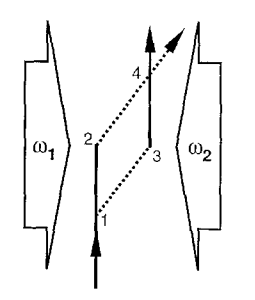
\includegraphics[width=0.23\textwidth]{MZI.png}
	\caption{Lines show the mean paths of an atom in an MZ atom interferometer. The solid (dash) lines correspond to the ground (excited) state of the atom. $\omega_1,\omega_2$ are the angular frequencies of the laser fields. From \cite{kasevich1992measurement}.}
	\label{fig:MZI}
\end{figure}


As is the case in optical interferometers where longer arm lengths increase the instrument's sensitivity, in atom interferometers the larger the wavepacket separation $\hbar k T /m$ the better. However, there is a trade-off between drift time and recoil velocities. Drift times on the order of 1s generally require metastable atomic transitions. While hyperfine transitions fulfill this requirement, the recoil velocities are small ($0.1 \, \mu\text{m/s}$ for $F=1, 3S_{1/2}\to F=2,3S_{1/2}$ in Na). Conversely, metastable optical transitions have large recoil velocities, but often need ultra-stable lasers to drive \cite{kasevich1992measurement}. The methods described in the forthcoming subsections \ref{sect:SRT} and \ref{sect:BD} circumvent this issue. 



\subsection{Stimulated Raman Transitions}\label{sect:SRT}



Stimulated Raman Transitions is one of the first techniques developed for obtaining large recoil while simultaneously meeting the metastability criterion. The following treatment\footnote{Pset\#12 of 8.421, Spring 2022, treats this problem in a slightly different approach.} of the theory is due to \cite{kasevich1992measurement}. The Hamiltonian for the three-level system is 
\begin{align*}
\mathcal{H} = \f{\vec{p}\,^2}{2m} + \hbar \omega_1^A \ketbra{1} + \hbar \omega_2^A \ketbra{2} + \hbar \omega_i^A \ketbra{i} - e\vec{r}\cdot \vec{E}
\end{align*}
where
\begin{align*}
\vec{E} = \vec{E}_1 \cos(k_1 x - \omega_1 t + \Phi_1) + \vec{E}_2 \cos(k_2 x - \omega_2 t + \Phi_2),
\end{align*}
describing the electric field due to two laser fields. Here, the superscript ``A'' denotes ``atom.'' $\omega_1, \omega_2 \sim \omega^A_i - \omega_1^A$, and $\omega_1 - \omega_2 \sim \omega_2^A - \omega_1^A$ (see Figure \ref{fig:Raman}). For counter-propagating beams, $k_1 \sim -k_2$. We look for solutions to the Schr\"{o}dinger equation of the form 
\begin{align*}
\ket{\Psi} = \int dp\, \sum_\al a_{\al,p}(t) e^{-i(\omega_\al^A + p^2/2m) t } \ket{\al,p}
\end{align*}
where $\ket{\al,p}$ denotes an atom in internal state $\ket{\al}$ and momentum eigenstate $ \phi_p(x) \sim e^{ipx/\hbar}$. For a given $p$, the Schr\"{o}dinger equation after the rotating wave approximation reduces to 
\begin{align*}
\dot{a}_{1,p} &= \f{i}{2}e^{i\Delta_1 t} \Omega^*_{1i} a_{i,p+\hbar k_1}\\
\dot{a}_{i,p + \hbar k_1} &= \f{i}{2}\lb \Omega_{i1}e^{-i\Delta_1 t } a_{1,p}+ \Omega_{i2} e^{-i\Delta_2 t}a_{2,p+\hbar k_1 - \hbar k_2} \rb \\
\dot{a}_{2,p+\hbar k_1 - \hbar k_2} &= \f{i}{2}e^{i\Delta_2 t}\Omega_{1i}^* a_{i,p+\hbar k_1},
\end{align*}
where we have assumed that the electric field $\vec{E}_j$ only couples to the $\ket{j} \to \ket{i}$ transitions and 
\begin{align*}
\Omega_{ji} &= e\bra{i} \vec{r}\cdot \vec{E}_j \ket{j} e^{i\Phi_j}/\hbar\\
\Delta_j &= (\omega_j^A + \omega_j - \omega_i^A) + p_j^2/2m - p_i^2/2m
\end{align*}
with $j=1,2$ and $i$ denotes the intermediate state. Adiabatically eliminating\footnote{Adiabatic elimination is a tool in quantum optics often used to extract effective two-level dynamics from a three-level system driven by off-resonant light. See \cite{brion2007adiabatic}.} $\ket{i}$ and setting $p_1 = p, p_2 = p+ \hbar k_1 - \hbar k_2$ give 
\begin{align}
\dot{a}_{1,p_1} &\approx -\f{i}{2}\Omega_1^{\text{AC}} a_{1,p_1} - \f{i}{2}e^{i\delta_{12} t} \Omega_\text{eff} a_{2,p_2}\label{eq:raman1}\\
\dot{a}_{2,p_2} &\approx -\f{i}{2}\Omega_2^{\text{AC}} a_{2,p_2} - \f{i}{2}e^{-i\delta_{12} t} \Omega_{\text{eff}}^* a_{1,p_1}\label{eq:raman2},
\end{align}
where  
\begin{align*}
\Omega_\text{eff} &= \Omega_{1i}^* \Omega_{i2}/2\Delta, \quad \Omega_j^{\text{AC}} = |\Omega_{ji}|^2/2\Delta, \quad \text{and}\\
\delta_{12} &= (\omega_1 - \omega_2) - (\omega_2^A - \omega_1^A)\\
&\quad- \lb  v_x(k_1-k_2) + \f{\hbar (k_1 - k_2)^2}{ m} \rb.
\end{align*}
Here $v_x$ is the velocity of the atoms along the beams. The first terms on the right of \eqref{eq:raman1} and \eqref{eq:raman2} correspond to AC Stark shifts. The second terms correspond to Rabi flopping between the two levels. The effective detuning $\delta_{12}$ from the Raman resonance contains the AC Stark shifts, Doppler shifts, and recoil shifts. A resonant process transfers an atom initially in $\ket{1,\bm{p}}$ to $\ket{2, \bm{p} + \hbar \bm{k}_1 - \hbar \bm{k}_2}$. Figure \ref{fig:Raman} shows the relevant parameters for this process. 
 

\begin{figure}
	\subfigure[]{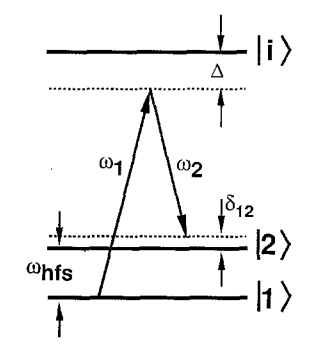
\includegraphics[width=0.23\textwidth]{Raman.png}}\quad
	\subfigure[]{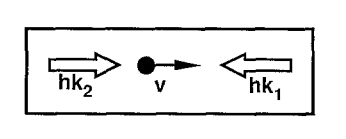
\includegraphics[width=0.23\textwidth]{Raman1.png}}
	\caption{(a) Energy diagram for stimulated Raman transitions between $\ket{1}$ and $\ket{2}$. Raman beams are detuned by $\Delta$ from the transitions to $\ket{i}$. $\delta_{12}$ is velocity-dependent. Following $\ket{1} \to \ket{2}$, the atom's momentum changes by $\hbar \bm{k}_1 - \hbar \bm{k}_2$. (b) Geometry for the velocity-selective configuration. From \cite{kasevich1992measurement}.}
	\label{fig:Raman}
\end{figure}




\subsection{Bragg Diffraction}\label{sect:BD}


Bragg diffraction, partially invented and developed by the Holger M\"{u}ller group at UC Berkeley, is another tool for generating large momentum transfers for atom interferometry. It may be viewed as an improvement over the two-photon stimulated Raman process since an atom generally absorbs the momentum of more than two photons while remaining in its electronic ground state.  The following treatment of Bragg diffraction is due to \cite{estey2016precision}. Let $\omega_0$ be the transition frequency between $\ket{g}$ and $\ket{e}$ and $\Omega \equiv \vec{d}_\text{ge}\cdot \vec{E}_0/\hbar$ be the Rabi frequency, where $\vec{d}_\text{ge}$ is the dipole matrix element of the atom. For generalized electric fields, $\vec{E} = \sum_j \vec{E}_j \cos(k_j z - (\omega_L - \delta_j)t)$, the Hamiltonian in the rotating frame is
\begin{align*}
\mathcal{H}^\text{rot} = &\f{\vec{p}\,^2}{2m} - \hbar \Delta \ketbra{e} \\
&- \lp \sum_j \f{\hbar \Omega_j}{2} e^{ik_jz + i \delta_i t} \ket{e}\bra{g} + h.c. \rp,
\end{align*}
where $|\delta_j|\ll \omega_L$ are small detunings from the ``center'' frequency $\omega_L$ and $\Omega_j \equiv \vec{d}_\text{ge}\cdot \vec{E}_j / \hbar$. In Bragg diffraction, the electric field is a nearly-standing wave. After the rotating wave approximation, 
\begin{align*}
\vec{E} \to \f{\vec{E}_0}{2}u(z,t) = \f{\vec{E}_0}{2} \lp  e^{-ikz + i\delta t} + e^{ikz-i\delta t}\rp,
\end{align*}
where $2\delta$ is the detuning between the counter-propagating beams, and so
\begin{align*}
\mathcal{H}^\text{rot} = \f{\vec{p}\,^2}{2m} -\hbar \Delta  \ketbra{e} -\lp \f{\hbar\Omega u(z,t)}{2}\ket{e}\bra{g} + h.c.\rp.
\end{align*}
The solutions to this Hamiltonian have the form 
\begin{align*}
\ket{\Psi} = e(z,t)\ket{e} + g(z,t)\ket{g}.
\end{align*} 
From the Schr\"{o}dinger equation for $\ket{\Psi}$ with $\mathcal{H}^\text{rot}$, we get
\begin{align}
i\hbar \dot{e}(z,t) &= \f{\vec{p}\,^2}{2m} e(z,t) - \hbar \Delta e(z,t) - \f{\hbar\Omega}{2}ug(z,t)\label{eq:2}\\
i\hbar \dot{g}(z,t) &= \f{\vec{p}\,^2}{2m} g(z,t) - \f{\hbar\Omega^*}{2}u^*e(z,t)\label{eq:3}.
\end{align}
Since $\Delta \gg \Omega$, we may set $\dot{e}(z,t) = 0$ by adiabatic elimination. Moreover, $\Delta \gg \omega_r = \hbar k^2/2m$, the recoil frequency, and so $\vec{p}\,^2/2m\ll \hbar \Delta$ in \eqref{eq:2}. Solving for $e(z,t)$ and substituting into \eqref{eq:3} gives
\begin{align}\label{eq:de}
i\dot{g}(z,t) = -\f{\hbar}{2m}\p_z^2 g(z,t) + \f{|\Omega|^2}{4\Delta} uu^* g(z,t).
\end{align}
Since the electric field $\sim u(z,t)$ is periodic, we may choose the following ansatz for $g(z,t)$\footnote{This is equivalent to the ansatz in \ref{sect:SRT}.}:
\begin{align}\label{eq:ansatz}
g(z,t) = \sum_{-\infty}^\infty g_n(t) e^{i2nkz} e^{-i(2n)^2 \omega_r t}.
\end{align}
Inserting this ansatz into \eqref{eq:de} and simplifying\footnote{See \cite{estey2016precision} for details regarding this step.},
\begin{align}\label{eq:soln}
i\dot{g}_n = &\f{\bar{\Omega}}{2} g_{n+1} e^{i2\delta t} e^{-i 4(2n+1) \omega_r t} \nonumber\\
&\quad+ \f{\bar{\Omega}}{2}g_{n-1} e^{-i2\delta t} e^{i4(2n-1)\omega_r t},
\end{align}
where $\bar{\Omega} = |\Omega|^2/2\Delta$ is the two-photon Rabi frequency. This is an infinite set of coupled differential equations where the plane wave momentum states of the atom are coupled only by integer multiples of the photon momentum $\hbar k$. An atom starting in $g_{n_I}$ with momentum $2n_I \hbar k$ can only be transferred to $g_{n_F}$ with momentum $2n_F \hbar k$. The Bragg resonance condition for this process is $\delta = 2(n_F + n_I)\omega_r$.   To solve this system in practice, we consider the case where an atom initially in a pure momentum state $g_{n_I} = 1$ is resonantly transferred to a state $g_{n_F}$ via $\delta = 2(n_I + n_F)\omega_r$. For sufficiently long interaction times, terms proportional to $e^{i4(\pm 2j \pm  1)}$ for $|j|\gg n$ oscillate rapidly and may be taken to be zero. We can then choose cutoffs $n_+ > \max(n_I, n_F)$ and $-n_- < \min(n_I, n_F)$ so that \eqref{eq:soln} reduces to a  finite system 
%\begin{align*}
%i\dot{g}_{n_++1} &= 0\\
%%i\dot{g}_{n_+} &= \f{\bar{\Omega}}{2}\lb g_{n_+ - 1} e^{-i2\delta t} e^{i4(2n_+-1)\omega_r t}\rb\\
%%i\dot{g}_{n_+ - 1} &= \f{\bar{\Omega}}{2} g_{n_+} e^{i2\delta t} e^{-i4(2n_+-1)\omega_r t}\\ 
%%&\quad+ \f{\bar{\Omega}}{2}g_{n_+-2} e^{-i2\delta t} e^{i4(2n_+-3)\omega_rt}\\
%&\vdots\\
%i\dot{g}_{n} &= \f{\bar{\Omega}}{2} g_{n+1} e^{i2\delta t} e^{-i4(2n+1)\omega_r t}\\ 
%&\quad+ \f{\bar{\Omega}}{2}g_{n-1} e^{-i2\delta t} e^{i4(2n-1)\omega_rt}\\
%&\vdots\\
%%i\dot{g}_{-n_- + 1} &= \f{\bar{\Omega}}{2} g_{-n_-+2} e^{i2\delta t} e^{-i4(-2n_-+3)\omega_r t}\\ 
%%&\quad+ \f{\bar{\Omega}}{2}g_{-n_-} e^{-i2\delta t} e^{i4(-2n_-+1)\omega_rt}\\
%%i\dot{g}_{-n_-} &= \f{\bar{\Omega}}{2}\lb g_{-n_- + 1} e^{i2\delta t} e^{-i4(-2n_-+1)\omega_r t}\rb\\
%i\dot{g}_{-n_--1} &= 0,
%\end{align*}
which can be solved numerically. 



Figure \ref{fig:Bragg} shows the relevant momentum states of an atom and laser fields for Bragg diffraction, transferring atoms from $\ket{g,0\hbar k}$ to $\ket{g,6\hbar k}$. The detuning of the undesired $2m$-photon process $\ket{g,0\hbar k} \to \ket{g,2m\hbar k}$ is $2m\delta - 4m^2 \omega_r$. For the undesired intermediate states (solid blue, $m\neq n$) to remain unpopulated, $\delta_m$ for $m\neq n$ must be much greater than $\bar{\Omega}$. In practice, efficient transfers are determined by a number of factors including the time-dependence of the two-photon Rabi frequency, pulse width, shape, and the momentum spread of the atoms. A detailed discussion of these parameters in \cite{estey2016precision} is beyond the scope of this paper, but it is important to mention the last point regarding moving atoms. We so far have been confined to the case where the atoms are at rest relative to the standing wave $(\delta = 0)$ caused by the Bragg beams. When $g_0(t)$ has some velocity $\Delta v$, the ansatz \eqref{eq:ansatz} is modified, and the system of equations becomes
\begin{align*}
i\dot{g}_n &= \f{\bar{\Omega}}{2}\lb g_{n+1} e^{i2(\delta - 2\omega_r \Delta v/v_r)t} e^{-i4(2n+1)\omega_r t} \rb \\ 
& \quad + \f{\bar{\Omega}}{2}g_{n-1} e^{-i2(\delta - 2\omega_r \Delta v/v_r) t} e^{i4(2n-1)\omega_r t} ,
\end{align*}
where $v_r = \hbar k/m$ is the recoil velocity. In this case atoms with net velocity $\Delta v$ are out of resonance with the Bragg condition $\delta = 2(n_F + n_I)\omega_r$ by $2\omega_r \Delta / v_r$, but still only couple to higher or lower momentum states by multiples of $2\hbar k$. This is important since atoms for real interferometers always have some finite velocity distribution. 

\begin{figure}
	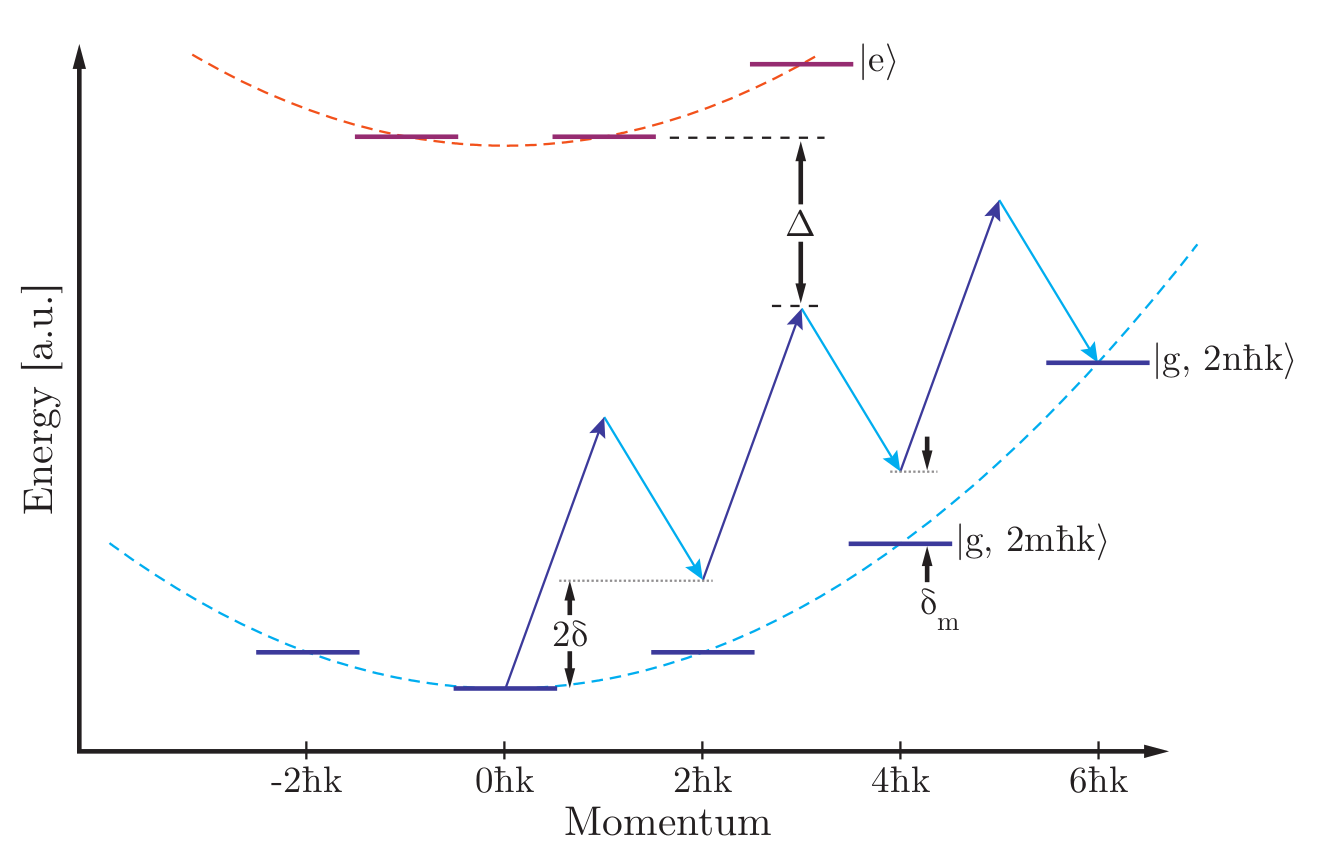
\includegraphics[width=0.47\textwidth]{Bragg.png}
	\caption{Relevant momentum states of an atom and laser fields for Bragg diffraction. $2\delta$ is the detuning between counter-propagating Bragg beams. $\Delta$ is the single-photon detuning of the lasers from $\ket{e}$. $\delta_m$ is the multi-photon detuning to an arbitrary intermediate ground state $\ket{g,m\hbar k}$. From \cite{estey2016precision}.}
	\label{fig:Bragg}
\end{figure}



\section{Observation of a Gravitational Aharonov-Bohm Effect}\label{sect:grav}
Several experimental verifications of the Aharonov-Bohm effect and the existence of the Berry phase have been realized since their theoretical conceptions (\cite{tonomura1986evidence}, \cite{cimmino1989observation}). However, these experiments, which were conducted around the 1980s-1990s, have exclusively been in the electromagnetic domain and used electrons and neutrons rather than neutral atoms as matter-wave sources. Similar measurements for the much weaker gravitational analogue have only been possible more recently due to advances in light-pulse atom interferometers and growing interests in their role as ultraprecise quantum sensors \cite{bongs2019taking}, for which a notable example is the measurement of the gravitational acceleration to $3\times 10^{-8} g$ by M. Kasevich and S. Chu \cite{kasevich1992measurement}. 


In 2018, H. M\"{u}ller and colleagues proposed an experiment for measuring the gravitational analogue of the Aharonov-Bohm effect \cite{hohensee2012force}. The setup  
consists of two identical spheres whose combined gravitational potential has a saddle point $x_A$ between the spheres and two other points $\pm x_B$ near the spheres' centers. Atoms of mass $m$ in the two arms of a Mach-Zehnder interferometer are moved to the two saddle points $x_A,x_B$ by a moving optical lattice and spend a sufficiently long time $T = t_2- t_1$ there, during which they accumulate phase shifts $\phi_A, \phi_B$. When the states are interfered at $t_3$, the phase difference $\Delta \phi = \phi_A - \phi_B$ is measured by detecting the population in the outputs of the interferometer, which is given by $\cos^2\Delta \phi/2$. The contribution to $\Delta \phi$ due to the gravitational Aharonov-Bohm effect, $\delta \phi_G$, is given by $m\Delta U T/\hbar$, where $\Delta U$ is the potential difference between $x_A$ and $x_B$.  While plausible, this proposal has not been realized since perturbations in the optical lattice required to transport and suspend the atoms in the Earth's gravitational field would contaminate the interference signal \cite{roura2022quantum}.  


%\begin{figure}
%	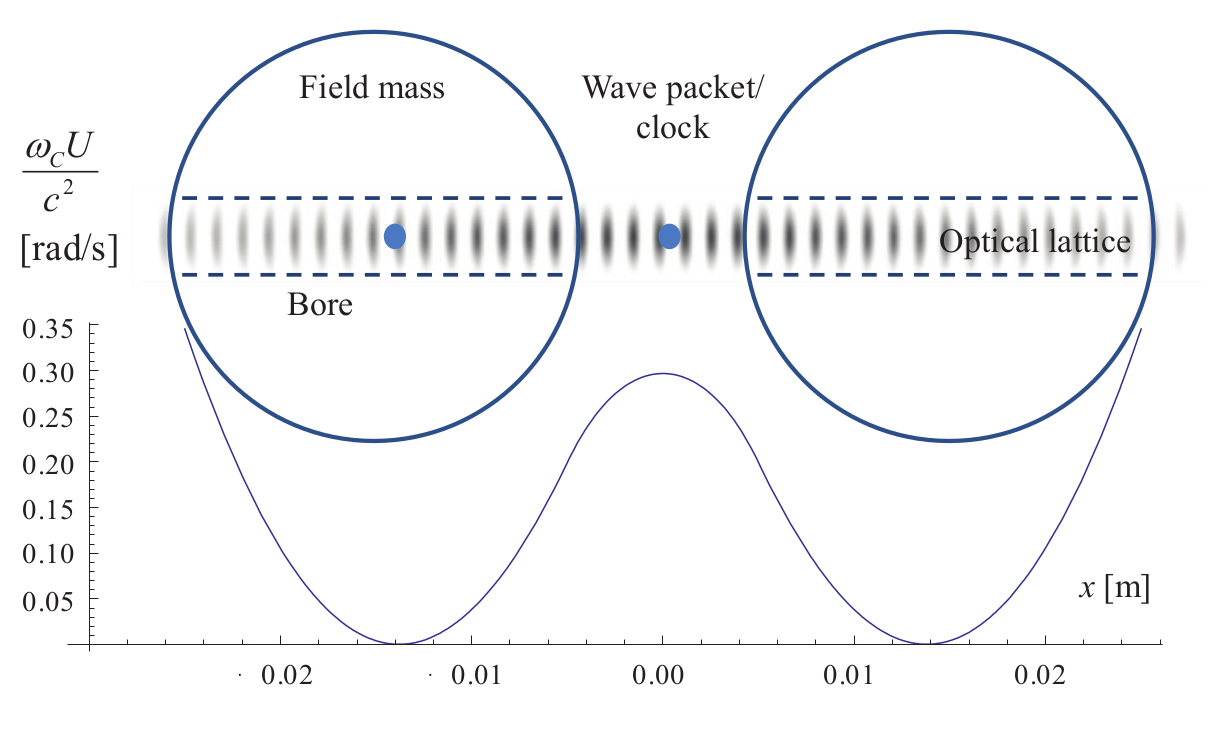
\includegraphics[width=0.35\textwidth]{proposal.png}
%	\caption{Blah. From \cite{hohensee2012force}}
%	\label{fig:proposal}
%\end{figure}








\subsection{Observation of the gravitational Aharonov-Bohm effect}


In their recent work \cite{overstreet2022observation}, Overstreet \textit{et al.} used an atom interferometer in a ``fountain'' configuration, as shown in Figure \ref{fig:overstreet1}, which does not require an optical lattice for suspending atoms during the phase accumulation stage.  A simplified\footnote{In the experiment, two interferometers are used, with one serving as a reference for removing contributions to the phase shift due to phase fluctuations in the laser fields. The interferometer also has components to account for deflections in the atom trajectories due to gravitational effects.} description of their experiment is as follows: $^{87}$Rb atoms at $1$ $\mu$K are launched into a 10-m vacuum tube by an optical lattice. The matter-wave beamsplitters and mirrors transfer momentum to the atoms via Bragg diffraction, the process described in Section \ref{sect:BD}.  Here, the Bragg beamsplitter pulse creates large momentum transfers $(52\hbar k)$ and wavepacket separation ($25$ cm), enhancing the sensitivity to the gravitational effect of a tungsten mass at the top of the tube. The atoms receiving the 52$\hbar k$ momentum kick travel upwards to a distance $R_x$ from the tungsten mass and interact with it more strongly than the atoms without the momentum kick. Finally, a mirror pulse and a subsequent beamsplitter pulse redirect and recombine the atoms and allow them to interfere. The atoms are then imaged by resonant scattering, and the interference pattern is observed. The measured phase shifts are in good agreement with ab-initio quantum mechanical calculations (see Figure \ref{fig:data}). 






\begin{figure}
	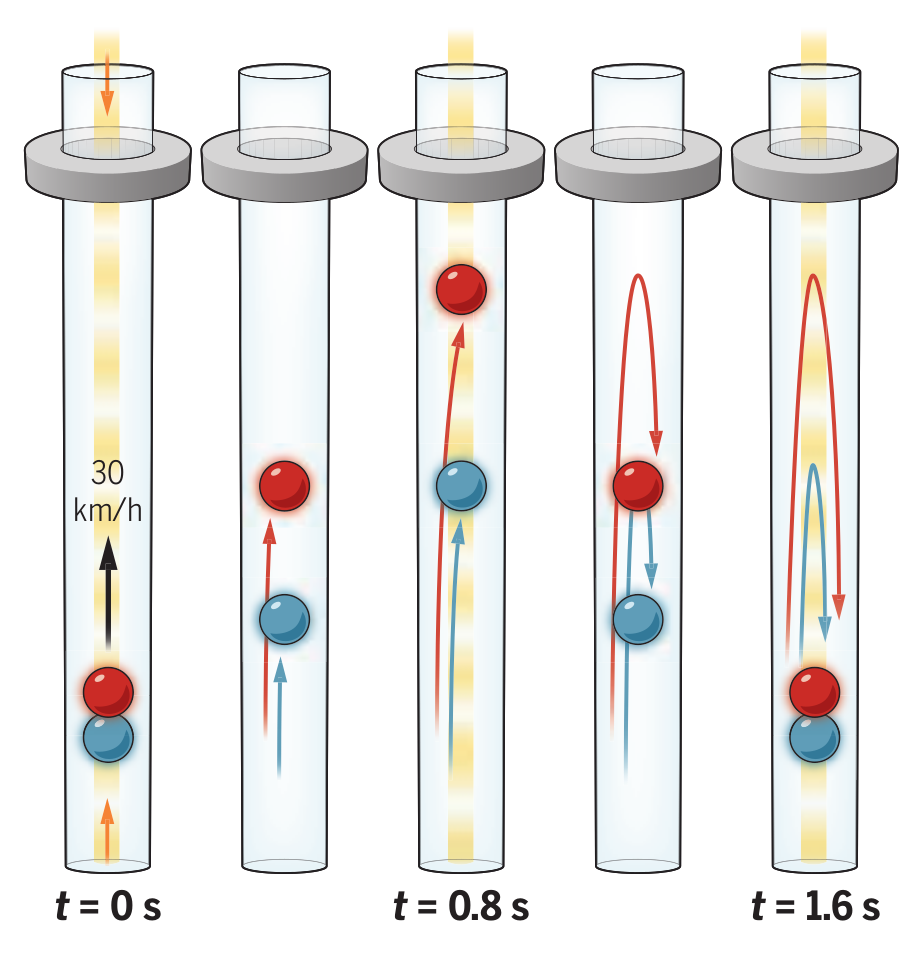
\includegraphics[width=0.29\textwidth]{overstreet1.png}
	\caption{A fountain Mach-Zehnder atom interferometer. $^{87}$Rb atoms are launched vertically from the bottom of a 10-meter vacuum tube and follow a free-fall trajectory. Laser pulses were applied at three different times to split, redirect, and recombine the wavepackets. The gravitational influence of the ring mass on the upper inteferometer arm is measured from the interference signal. From \cite{roura2022quantum}.}
	\label{fig:overstreet1}
\end{figure}




\begin{figure}
	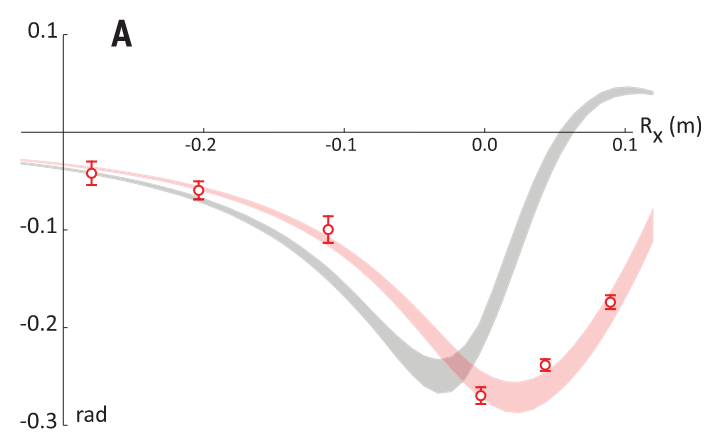
\includegraphics[width=0.45\textwidth]{52hbark_edited.png}
	\caption{Plot of the phase shift induced by the tungsten mass as a function of $R_x$. The red and gray curves are theoretical predictions. From \cite{overstreet2022observation}.}
	\label{fig:data}
\end{figure}







\section{Conclusions}


In this paper, we re-introduce the notion of the Berry phase and interpret the Aharonov-Bohm effect as an example. Mirroring the role of matter-wave interferometers in the experimental verification of the magnetic Aharonov-Bohm effect, light-pulse atom interferometers have recently measured the much weaker gravitational analogue of this effect. In our brief introduction to atom interferometry, we review two atom-light interactions, namely the stimulated Raman transitions and Bragg diffraction, which are the key ingredients to the workings of modern light-pulse atom interferometers. The field of atom interferometry is incredibly rich with theory and experimental techniques which are vastly beyond the scope of this paper. However, the author hopes that this paper can serve as a good starting point for those interested in the subject. 



\begin{acknowledgments}
	The author would like to thank Professor Zwierlein for his exciting AMO I lectures. 8.421 is the first \textit{official} course in atomic physics for the author, and he looks forward to continuing his studies in 8.422: AMO II. 
\end{acknowledgments}


\bibliographystyle{apsrev4-1}
\bibliography{HuanBui_AMO_refs}% Produces the bibliography via BibTeX.











\end{document}
